\documentclass{beamer}
\usepackage[utf8]{inputenc}

\usetheme{Madrid}
\usecolortheme{default}
\usepackage{amsmath,amssymb,amsfonts,amsthm}
\usepackage{txfonts}
\usepackage{tkz-euclide}
\usepackage{listings}
\usepackage{adjustbox}
\usepackage{array}
\usepackage{tabularx}
\usepackage{gvv}
\usepackage{lmodern}
\usepackage{circuitikz}
\usepackage{tikz}
\usepackage{graphicx}
\usepackage{mathtools}
\setbeamertemplate{page number in head/foot}[totalframenumber]

\usepackage{tcolorbox}
\tcbuselibrary{minted,breakable,xparse,skins}



\definecolor{bg}{gray}{0.95}
\DeclareTCBListing{mintedbox}{O{}m!O{}}{%
  breakable=true,
  listing engine=minted,
  listing only,
  minted language=#2,
  minted style=default,
  minted options={%
    linenos,
    gobble=0,
    breaklines=true,
    breakafter=,,
    fontsize=\small,
    numbersep=8pt,
    #1},
  boxsep=0pt,
  left skip=0pt,
  right skip=0pt,
  left=25pt,
  right=0pt,
  top=3pt,
  bottom=3pt,
  arc=5pt,
  leftrule=0pt,
  rightrule=0pt,
  bottomrule=2pt,
  toprule=2pt,
  colback=bg,
  colframe=orange!70,
  enhanced,
  overlay={%
    \begin{tcbclipinterior}
    \fill[orange!20!white] (frame.south west) rectangle ([xshift=20pt]frame.north west);
    \end{tcbclipinterior}},
  #3,
}
\lstset{
    language=C,
    basicstyle=\ttfamily\small,
    keywordstyle=\color{blue},
    stringstyle=\color{orange},
    commentstyle=\color{green!60!black},
    numbers=left,
    numberstyle=\tiny\color{gray},
    breaklines=true,
    showstringspaces=false,
}


\title 
{4.8.3}


\author 
{AI25BTECH11008- Chiruvella Harshith Sharan}



\begin{document}
\frame{\titlepage}
\begin{frame}{Question}
Find the equation of the plane passing through the points 
$A(2, 5, -3), B(-2, -3, 5)$ and $C(5, 3, -3)$.
\end{frame}
\begin{frame}{Solution}
\begin{align}
\vec{A} &= \myvec{2 \\ 5 \\ -3}, & 
\vec{B} &= \myvec{-2 \\ -3 \\ 5}, & 
\vec{C} &= \myvec{5 \\ 3 \\ -3}.
\end{align}

Let the equation of the plane be
\begin{align}
\vec{n}^T \vec{x} &= 1.
\end{align}

Since $\vec{A}, \vec{B}, \vec{C}$ lie in the plane:
\begin{align}
\vec{n}^T \vec{A} &= 1, & 
\vec{n}^T \vec{B} &= 1, & 
\vec{n}^T \vec{C} &= 1,
\end{align}
or equivalently
\end{frame}
\begin{frame}{Solution}

\begin{align}
\vec{A}^T \vec{n} &= 1, & 
\vec{B}^T \vec{n} &= 1, & 
\vec{C}^T \vec{n} &= 1.
\end{align}

Hence,


\begin{align}
\myvec{\vec{A} & \vec{B} & \vec{C}}^{T} \vec{n} 
&= 1.
\end{align}
\

\begin{align}
\myvec{ 2 & 5 & -3 \\ -2 & -3 & 5 \\ 5 & 3 & -3}\vec{n}
&= \myvec{1 \\ 1 \\ 1}.
\end{align}
\end{frame}
\begin{frame}{Solution}

Performing row operations:
\begin{align}
R_2 &\leftarrow R_2 + R_1, \\
\myvec{2 & 5 & -3 \\ 0 & 2 & 2 \\ 5 & 3 & -3}\vec{n}
&= \myvec{1 \\ 2 \\ 1},\\
R_3 &\leftarrow 2R_3 - 5R_1, \\
\myvec{2 & 5 & -3 \\ 0 & 2 & 2 \\ 0 & -19 & 9}\vec{n}
&= \myvec{1 \\ 2 \\ -3},\\
R_3 &\leftarrow 19R_2 + 2R_3, \\
\myvec{2 & 5 & -3 \\ 0 & 2 & 2 \\ 0 & 0 & 56}\vec{n}
&= \myvec{1 \\ 2 \\ 32}.
\end{align}
\end{frame}
\begin{frame}{Solution}

Thus, solving we get
\begin{align}
\vec{n} = \myvec{\tfrac{2}{7} \\ \tfrac{3}{7} \\ \tfrac{4}{7}}.
\end{align}
Therfore,
The equation of plane is
\begin{align}
	\myvec{\tfrac{2}{7} \\ \tfrac{3}{7} \\ \tfrac{4}{7}}^T\vec{x} &= 1.
\end{align}
\end{frame}
\begin{frame}[fragile]                            
\frametitle{Python code  }                
\begin{lstlisting}
import numpy as np
from fractions import Fraction
import matplotlib.pyplot as plt
import os

# Create figs folder if it doesn't exist
os.makedirs("figs", exist_ok=True)

# Define points
A = np.array([2, 5, -3])
B = np.array([-2, -3, 5])
C = np.array([5, 3, -3])

# Coefficient matrix
M = np.array([A, B, C])
b = np.array([1, 1, 1])
\end{lstlisting}
\end{frame}
\begin{frame}[fragile]                            
\frametitle{Python code}                
\begin{lstlisting}

# Solve for normal vector n (float)
n_float = np.linalg.solve(M, b)

# Convert to fractions
n_frac = [Fraction(x).limit_denominator() for x in n_float]

# Display normal vector as column matrix
print("Normal vector n (column matrix in fractions):")
for val in n_frac:
    print(f"| {val} |")

# Plane equation in fraction form
x, y, z = 'x', 'y', 'z'
eq_terms = [f"{val}*{var}" for val, var in zip(n_frac, [x, y, z])]
plane_eq = " + ".join(eq_terms) + " = 1"
print("\nEquation of the plane (n^T x = 1) in fractions:")
print(plane_eq)

\end{lstlisting}
\end{frame}

\begin{frame}[fragile]                            
\frametitle{Python code}                
\begin{lstlisting}
# ----------------- Plotting -----------------
n1, n2, n3 = n_float  # Use float for plotting

# Create grid
xx = np.linspace(-5, 5, 20)
yy = np.linspace(-5, 5, 20)
X, Y = np.meshgrid(xx, yy)

# Solve for Z from plane equation
Z = (1 - n1*X - n2*Y) / n3
\end{lstlisting}
\end{frame}

\begin{frame}[fragile]                            
\frametitle{Python code}                
\begin{lstlisting}

# Plotting
fig = plt.figure(figsize=(8,6))
ax = fig.add_subplot(111, projection='3d')
ax.plot_surface(X, Y, Z, alpha=0.5, color='cyan', rstride=1, cstride=1)

# Plot points
points = {'A': A, 'B': B, 'C': C}
colors = {'A': 'red', 'B': 'green', 'C': 'blue'}

for label, point in points.items():
    ax.scatter(*point, color=colors[label], s=50, label=label)
    # Annotate with coordinates
    ax.text(point[0], point[1], point[2], f'{label}{tuple(point)}', color=colors[label])
\end{lstlisting}
\end{frame}

\begin{frame}[fragile]                            
\frametitle{Python code}                
\begin{lstlisting}

ax.set_xlabel('X')
ax.set_ylabel('Y')
ax.set_zlabel('Z')
ax.legend()
plt.title("Plane passing through points A, B, C")

# Save figure in figs folder
plt.savefig("figs/fig1.png")
plt.show()


\end{lstlisting}

\end{frame}


\begin{frame}[fragile]                            
\frametitle{C code}                
\begin{lstlisting}
#include <stdio.h>

typedef struct {
    double x, y, z;
} Point;

int main() {
    Point A = {2, 5, -3};
    Point B = {-2, -3, 5};
    Point C = {5, 3, -3};

    // Compute vectors AB and AC
    double AB[3] = {B.x - A.x, B.y - A.y, B.z - A.z};
    double AC[3] = {C.x - A.x, C.y - A.y, C.z - A.z};
\end{lstlisting}
\end{frame}

\begin{frame}[fragile]                            
\frametitle{C code}               
\begin{lstlisting}

    // Normal vector n = AB x AC
    double n[3];
    n[0] = AB[1]*AC[2] - AB[2]*AC[1];
    n[1] = AB[2]*AC[0] - AB[0]*AC[2];
    n[2] = AB[0]*AC[1] - AB[1]*AC[0];

    // Plane equation: n•X = d
    double d = n[0]*A.x + n[1]*A.y + n[2]*A.z;

    // Save points and plane to file
    FILE *fp = fopen("plane_points.dat", "w");
    fprintf(fp, "# Plane: %lf*x + %lf*y + %lf*z = %lf\n", n[0], n[1], n[2], d);
    fprintf(fp, "%lf %lf %lf\n", A.x, A.y, A.z);
    fprintf(fp, "%lf %lf %lf\n", B.x, B.y, B.z);
    fprintf(fp, "%lf %lf %lf\n", C.x, C.y, C.z);
    fclose(fp);
\end{lstlisting}
\end{frame}

\begin{frame}[fragile]                            
\frametitle{C code}               
\begin{lstlisting}

    // Print normal and d for Python
    printf("%lf %lf %lf %lf\n", n[0], n[1], n[2], d);

    return 0;
}


\end{lstlisting}
\end{frame}

\begin{frame}{Plot}
    \centering
    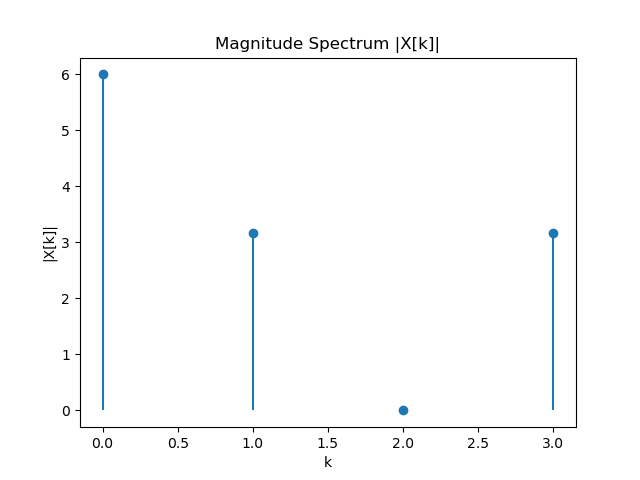
\includegraphics[width=\columnwidth, height=0.8\textheight, keepaspectratio]{beamer/figs/fig1.png}     
\end{frame}


	


\end{document}